\subsection{Opdracht 05a}
Geef ook het statement dat de langste reeks geeft die NIET in de database aanwezig is. Geef van beide statements het start en eind ID van de reeks.

\subsubsection{Versie 01}
In onderstaande query wordt er gebruik gemaakt van een CTE. Allereerst wordt de huidige ID vastgesteld. Vervolgens wordt er in deze
CTE gebruik gemaakt van een LAG functie, waardoor het verschil tussen de huidige ID en de vorige ID in de resultset kan worden vastgesteld.
Hierna wordt de grootte van dit verschil berekend door de vorige ID van de huidige ID af te trekken. Dit levert een waarde op welke
de maximale reeks met lege waarden bevat.
\lstinputlisting[language=SQL]{sql/marc/opdracht-01-05b.sql}
\begin{figure}[H]
    \centering
    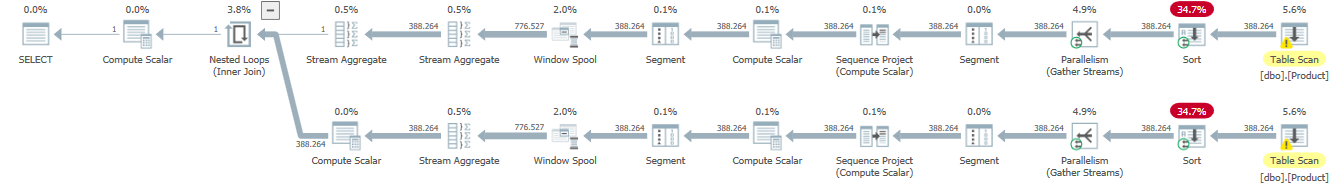
\includegraphics[width=1\textwidth]{image/marc/opdracht-05b.PNG}
    \caption{Queryplan Opdracht 05b Versie 01}
\end{figure}

\subsubsection{Versie 02}
TODO: Joey
\lstinputlisting[language=SQL]{sql/joey/opdracht-01-05b.sql}
\begin{figure}[H]
    \centering
    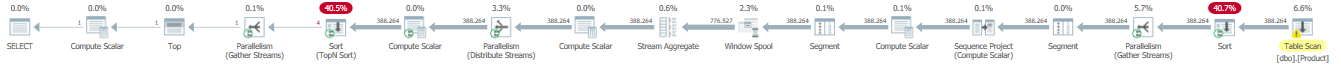
\includegraphics[width=1\textwidth]{image/joey/opdracht-05b.PNG}
    \caption{Queryplan Opdracht 05b Versie 02}
\end{figure}

\subsection{Conclusie}
Kijkende naar bovenstaande query plannen, kan worden gesteld dat versie 02 met 46\% net iets sneller is dan versie 01. In beide versies
is gebruik gemaakt van een CTE, in versie 01 wordt echter tweemaal gebruik gemaakt van de LAG functie om het verschil tussen de huidige
en de vorige rij in de resultset vast te stellen. Dit maakt deze query trager, wat ook blijkt uit het query plan. In het query plan van
versie 01 is te zien dat de LAG functie er tweemaal voor zorgt dat er een 'Tablescan' plaatsvind op de Product tabel. Deze gegevens worden
na deze 'Tablescan' allereerst gesorteerd middels een 'Sort'. Deze 'Sort' verbruikt beide keren 34,7\% van de query tijd, wat neer komt op
een totaal van 69,4\% van de gehele duur van de query. Ook versie 02 voert een 'Tablescan' op de Product tabel uit, echter wordt dit binnen
deze query maar één keer uitgevoerd. Hetzelfde geldt voor de hierop volgende 'Sort'.\\
\\
In versie 02 wordt er gebruik gemaakt van een TOP 1. Deze query is dus niet ANSI SQL. Bij versie 01 wordt op basis van de CTE het maximale
verschil vastgesteld.\\
\\
Gezien bovenstaande kan worden gesteld dat versie 01 in dit geval wellicht toch de beste optie is.
Wanneer beide queries in één batch worden uitgevoerd zijn de verschillen niet heel groot. Versie 01 is hierbij net wat trager, maar
voldoet wel aan de ANSI standaarden.\\
\\
\begin{tabular}{ || l | l | l | l | l | l | l | l | l | l | l | l | 1 | 1 | l | 1 | 1 || }
    \hline
    \textbf{Statement} & \textbf{Est Cost \%} & \textbf{Compile Time} & \textbf{Duration} &
    \textbf{CPU} & \textbf{Est CPU Cost \%} &
    \textbf{Est IO Cost \%} \\
    \hline
    \hline
    Versie01  & 54,0\%  & 12  & 1707  & 2370  & 52,6\% & 67,4\% \\
    \hline
    Versie02  & 46,0\%  & 8  & 958  & 1065  & 47,4\% & 67,4\%  \\
    \hline
\end{tabular}
\newline
\newline
\begin{tabular}{ || l | l | l | l | l | l | l | l | l | l | l | l | 1 | 1 | l | 1 | 1 || }
    \hline
    \textbf{Statement} &  \textbf{Est Rows} & \textbf{Actual Rows} & \textbf{RID Lookups} &
    \textbf{Parallel} & \textbf{Sort} &
    \textbf{Table Scan} & \textbf{Hash Match} \\
    \hline
    \hline
    Versie01  & 1  & 1  & 0  & 6  & 2  & 2  & 0 \\
    \hline
    Versie02  & 1  & 1  & 0  & 7  & 2  & 1  & 0 \\
    \hline
\end{tabular}